\documentclass{article}
\usepackage[utf8]{inputenc}

\usepackage{amsmath}
\usepackage{courier}
\usepackage[margin=1in]{geometry}
\usepackage{graphicx}
\usepackage{hyperref}
\usepackage{listings}
\usepackage{subcaption}
\usepackage{todonotes}
\usepackage[ruled]{algorithm2e}


\hypersetup{
    colorlinks=true,
    urlcolor=blue,
}

\lstset{basicstyle=\footnotesize\ttfamily, breaklines=true}

\title{Assignment 2: SIFT Local Feature Matching}
\author{CS 4476}
\date{Spring 2024}

\begin{document}

\maketitle

\section*{Brief}
\begin{itemize}
    \item{Due: Check \href{https://gatech.instructure.com/courses/366842}{Canvas} for up to date information}
    \item{Project materials including report template: \href{https://github.gatech.edu/vision}{Assignment 2}}
    \item{Hand-in: through \href{https://www.gradescope.com}{Gradescope}}
    \item{Required files: c\lstinline{<your_gt_username>.zip}, \lstinline{<your_gt_username>_proj2.pdf}}
\end{itemize}

\begin{figure}[h]
    \centering
    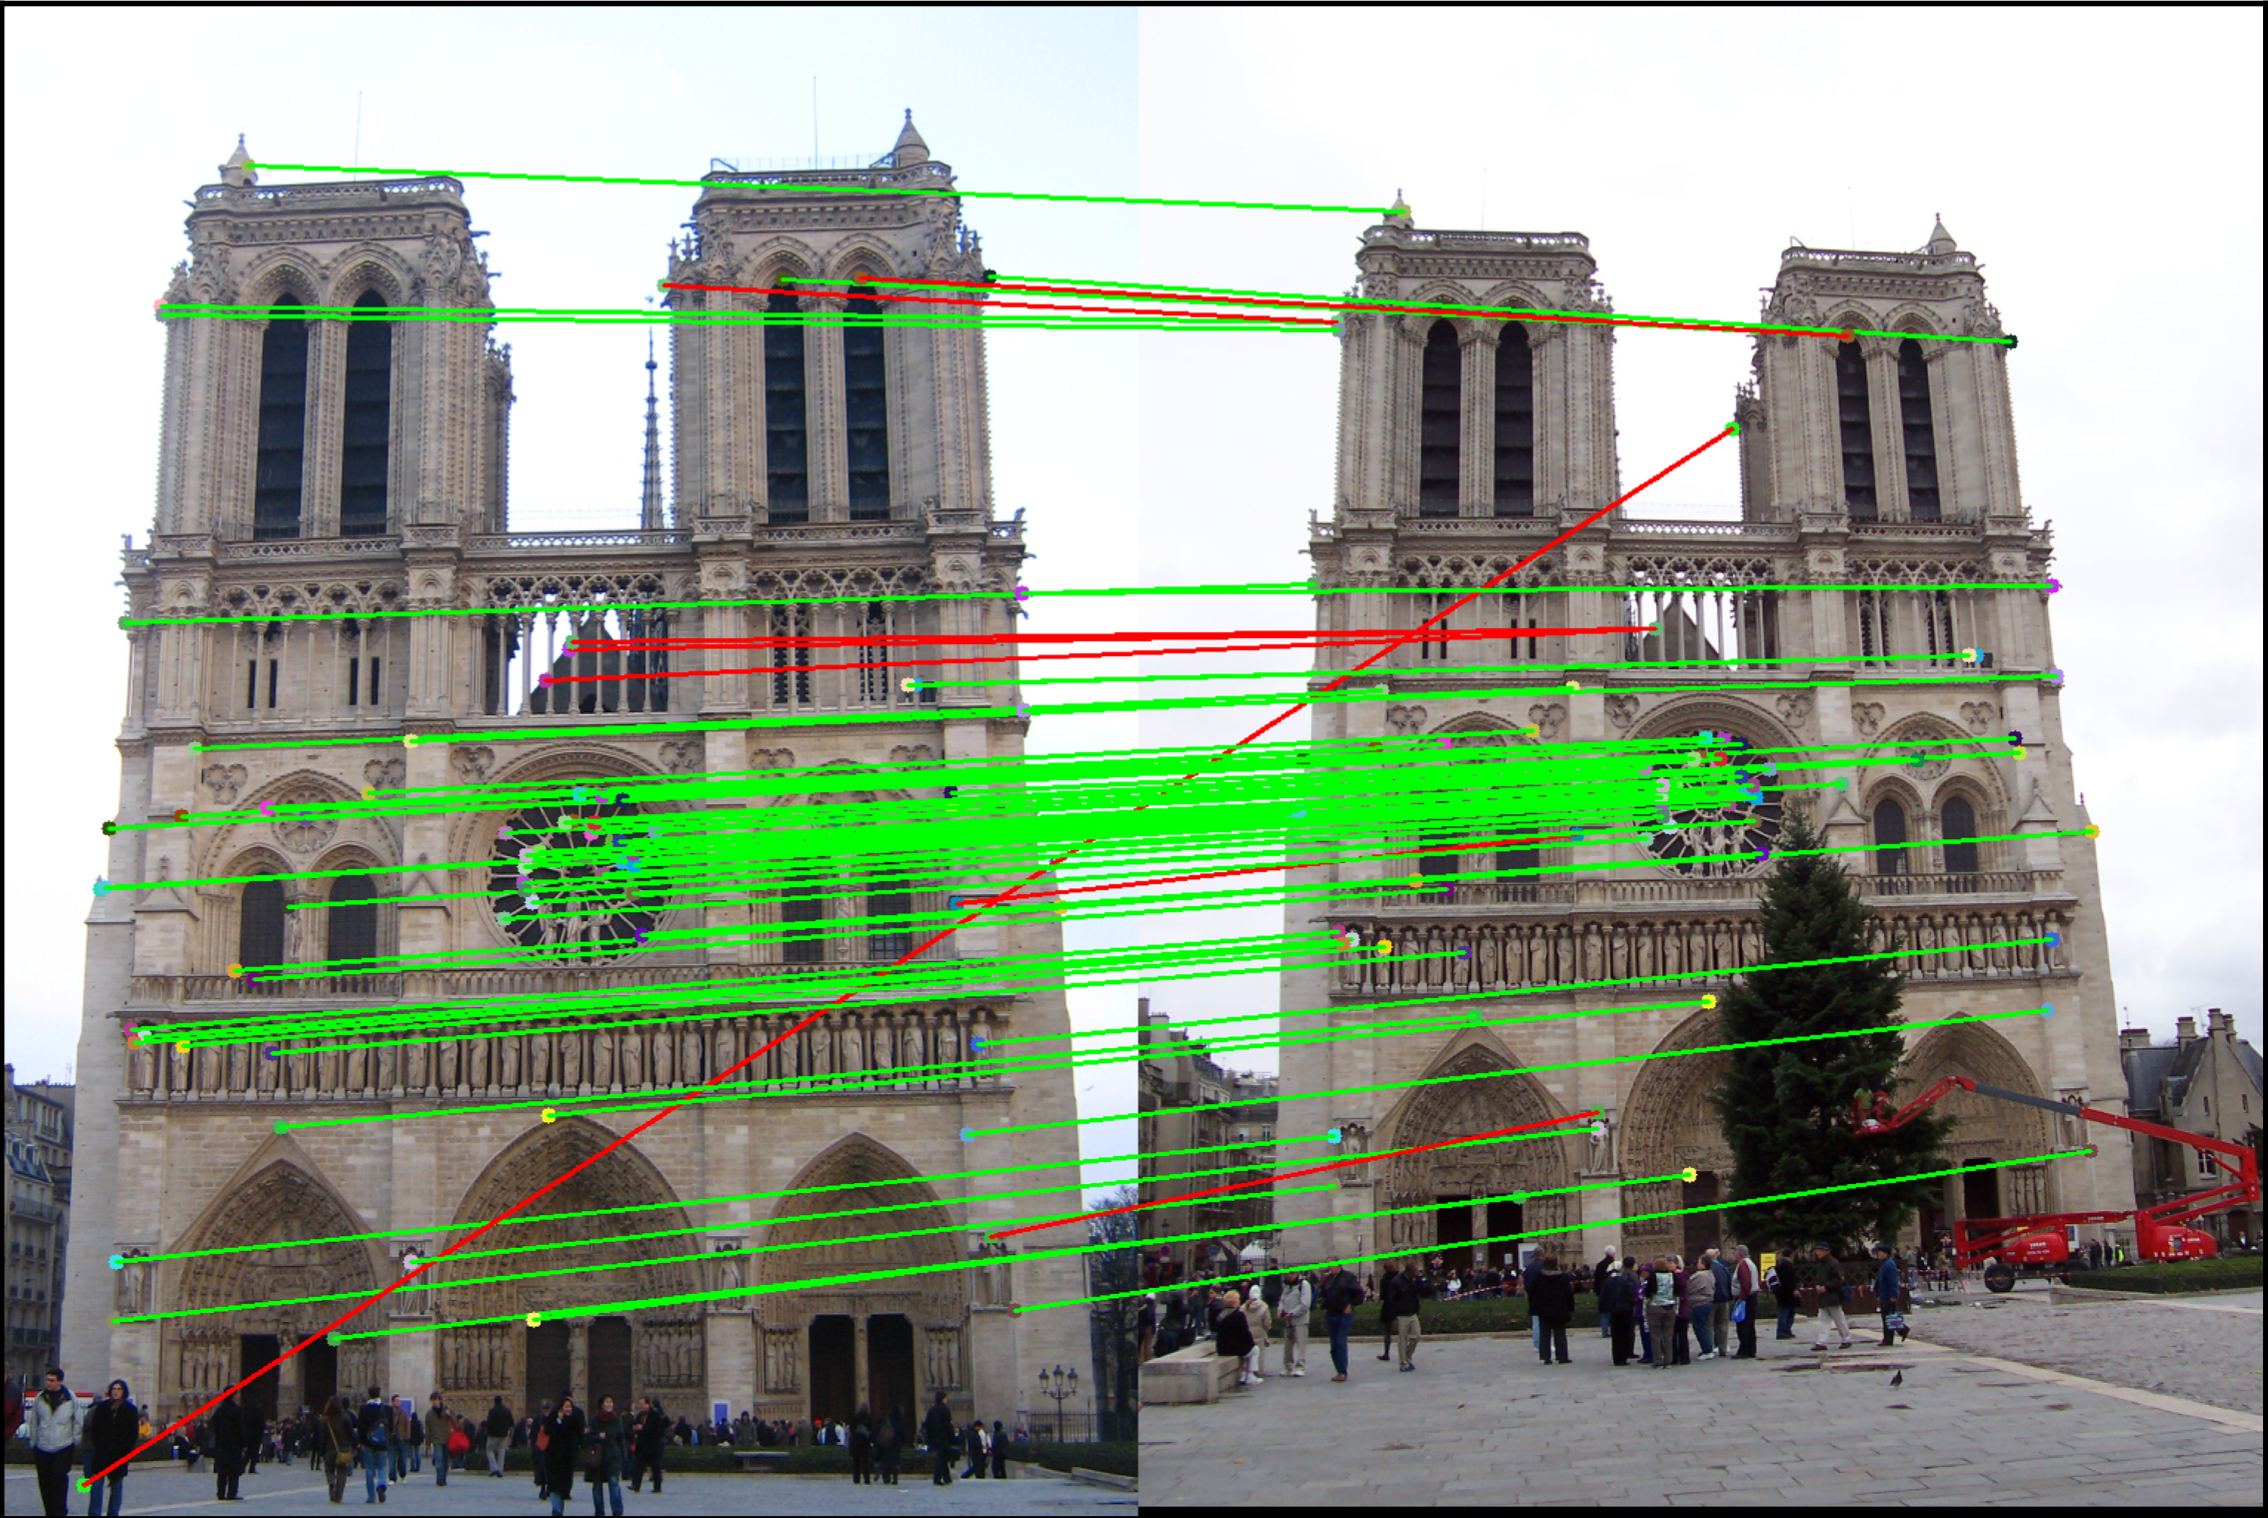
\includegraphics[width=\textwidth]{images/notre_dame.png}
    \caption{The top 100 most confident local feature matches from a baseline implementation of project 2. In this case, 89 were correct (lines shown in green), and 11 were incorrect (lines shown in red).}
    \label{fig:notre-dame}
\end{figure}


\section*{Overview}
The goal of this assignment is to create a local feature matching algorithm using techniques described in Szeliski chapter 7.1. The pipeline we suggest is a simplified version of the famous \href{https://www.cs.ubc.ca/~lowe/keypoints/}{SIFT} pipeline. The matching pipeline is intended to work for \textit{instance-level} matching -- multiple views of the same physical scene.


\section*{Setup}
\begin{enumerate}
    \item Check \href{https://github.gatech.edu/cs4476/project-2/blob/main/README.md}{https://github.gatech.edu/cs4476/project-2}. for environment installation.
    \item Run the notebook using \lstinline{jupyter notebook ./project-2.ipynb}
    \item After implementing all functions, ensure that all sanity checks are passing by running \lstinline{pytest tests} inside the main folder.
    \item Generate the zip folder for the code portion of your submission once you've finished the project using \lstinline{python zip_submission.py --gt_username <your_gt_username>}
\end{enumerate}


\section*{Details}
For this assignment, you need to implement the three major steps of a local feature matching algorithm (detecting interest points, creating local feature descriptors, and matching feature vectors). We'll implement two versions of the local feature descriptor, and the code is organized as follows:
\begin{itemize}
    \item{Interest point detection in \lstinline{part1_harris_corner.py} (see Szeliski 7.1.1)}
    \item{Local feature description with a simple normalized patch feature in \lstinline{part2_patch_descriptor.py} (see Szeliski 7.1.2)}
    \item{Feature matching in \lstinline{part3_feature_matching.py} (see Szeliski 7.1.3)}
    \item{Local feature description with the SIFT feature in \lstinline{part4_sift_descriptor.py} (see Szeliski 7.1.2) and comparison against Brute Force intensity-based matching.}
\end{itemize}

\section{Interest point detection (\lstinline{part1_harris_corner.py})}
You will implement the Harris corner detection as described in the lecture materials and Szeliski 7.1.1. 
\\
\\
The auto-correlation matrix $A$ can be computed as (Equation 7.8 of book, p. 424)
\begin{equation}
    A = w * \begin{bmatrix}
    I_x^2 & I_x I_y \\
    I_x I_y & I_y^2
    \end{bmatrix} = w * \begin{bmatrix}
    I_x \\ I_y 
    \end{bmatrix} \begin{bmatrix}
    I_x & I_y
    \end{bmatrix}
\end{equation}
where we have replaced the weighted summations with discrete convolutions with the weighting kernel $w$ (Equation 7.9, p. 425).
\\
\\
The Harris corner score $R$ is derived from the auto-correlation matrix $A$ as:
\begin{equation}
   R = \mbox{det}(A) - \alpha \cdot \mbox{trace}(A)^2 
\label{eqn:harris-corner-measure}
\end{equation}
with $\alpha=0.06$.

\begin{algorithm}[H]
\SetAlgoLined
% \KwResult{Write here the result }
 Compute the horizontal and vertical derivatives  $I_x$ and $I_y$ of the image by convolving the original image with a Sobel filter\;
 Compute the three images corresponding to the outer products of these gradients.
(The matrix A is symmetric, so only three entries are needed.)\;
Convolve each of these images with a larger Gaussian.\;
Compute a scalar interest measure using the formulas (Equation \ref{eqn:harris-corner-measure}) discussed above.\;
Find local maxima above a certain threshold and report them as detected feature
point locations.\;
 \caption{Harris Corner Detector}
\end{algorithm}

\noindent To implement the Harris corner detector, you will have to fill out the following methods in \lstinline{part1_harris_corner.py}:
\begin{itemize}
  \item \lstinline{compute_image_gradients()}: Computes image gradients using the Sobel filter.
  \item \lstinline{compute_harris_response_map()}: Gets the raw corner responses over the entire image (the previously implemented methods may be helpful).
  \item \lstinline{nms_maxpool_pytorch()}: Performs non-maximum suppression using max-pooling. You can use PyTorch max-pooling operations for this.
  \item \lstinline{get_harris_interest_points()}: Gets interests points from the entire image (the previously implemented methods may be helpful).
\end{itemize}
\noindent We have also provided the following helper methods in \lstinline{part1_harris_corner.py}:
\begin{itemize}
  \item \lstinline{get_gaussian_kernel_2D_pytorch()}: Creates a 2D Gaussian kernel (this is essentially the same as your Gaussian kernel method from project 1).
  \item \lstinline{second_moments()}: Computes the second moments of the input image. This makes use of your
  \lstinline{get_gaussian_kernel_2D_pytorch()} method.
  \item \lstinline{maxpool_numpy()}: Performs the maxpooling operation using just NumPy. This manual implementation will help you understand what's happening in the next step.
  \item \lstinline{remove_border_vals()}: Removes values close to the border that we can't create a useful SIFT window around. 
\end{itemize}
\\
The starter code gives some additional suggestions. You do not need to worry about scale invariance or keypoint orientation estimation for your baseline Harris corner detector. The original paper by Chris Harris and Mike Stephens describing their corner detector can be found \href{http://www.bmva.org/bmvc/1988/avc-88-023.pdf}{here}. 

\section{Part 2: Local feature descriptors (\lstinline{part2_patch_descriptor.py})}
To get your matching pipeline working quickly, you will implement a bare-bones feature descriptor in \lstinline{part2_patch_descriptor.py} using normalized, grayscale image intensity patches as your local feature. See Szeliski 7.1.2 for more details when coding \lstinline{compute_normalized_patch_descriptors()}
\\
\\
Choose the top-left option of the 4 possible choices for center of a square window, as shown in Figure \ref{fig:window}.

 \begin{figure}[h]
    \centering
    \includegraphics[width=150]{images/window.PNG}
    \caption{For this example of a $6\times6$ window, the yellow cells could all be considered the center. Please choose the top left (marked ``C'') as the center throughout this project.}
    \label{fig:window}
\end{figure}
\\
\\
The expected accuracy using Normalized patches on Notre Dame is around $40-45 \%$ and Mt Rushmore around $45-50 \%$.



\section{Part 3: Feature matching (\lstinline{part3_feature_matching.py})}
You will implement the ``ratio test'' (also known as the ``nearest neighbor distance ratio test'') method of matching local features as described in the lecture materials and Szeliski 7.1.3 (page 444). See equation 7.18 in particular. The potential matches that pass the ratio test the easiest should have a greater tendency to be correct matches -- think about \textit{why} this is. In \lstinline{part3_feature_matching.py}, you will have to code \lstinline{compute_feature_distances()} to get pairwise feature distances, and \lstinline{match_features_ratio_test()} to perform the ratio test to get matches from a pair of feature lists. 

\section{Part 4: SIFT vs Intensity-based Matching (\lstinline{part4_sift_descriptor.py})}

\subsection{SIFT local features}
You will implement a SIFT-like local feature as described in the lecture materials and Szeliski 7.1.2. We'll use a simple one-line modification (``Square-Root SIFT'') from a 2012 CVPR paper (\href{https://www.robots.ox.ac.uk/~vgg/publications/2012/Arandjelovic12/arandjelovic12.pdf}{linked here}) to get a free boost in performance. See the comments in the file \lstinline{part4_sift_descriptor.py} for more details.  \\ 

\noindent \textbf{Regarding Histograms}
SIFT relies upon histograms. An unweighted 1D histogram with 3 bins could have bin edges of $[0,2,4,6]$. If $x=[0.0, 0.1, 2.5, 5.8, 5.9]$, and the bins are defined over half-open intervals $[e_{left}, e_{right})$ with edges $e$, then the histogram $h = [2,1,2]$.
\\
\\
A weighted 1D histogram with the same 3 bins and bin edges has each item weighted by some value. For example, for an array $x=[0.0, 0.1, 2.5, 5.8, 5.9]$, with weights $w=[ 2, 3, 1, 0, 0]$, and the same bin edges ($[0,2,4,6]$), $h_w = [5, 1, 0]$. In SIFT, the histogram weight at a pixel is the magnitude of the image gradient at that pixel.
\\
\\
In \lstinline{part4_sift_descriptor.py}, you will have to implement the following:
\begin{itemize}
    \item \lstinline{get_magnitudes_and_orientations()}: Retrieves gradient magnitudes and orientations of the image.
    \item \lstinline{get_gradient_histogram_vec_from_patch()}: Retrieves a feature consisting of concatenated histograms.
    \item \lstinline{get_feat_vec()}: Gets the adjusted feature from a single point.
    \item \lstinline{get_SIFT_descriptors()}: Gets all feature vectors corresponding to our interest points from an image.
\end{itemize}
\\
The accuracy expected on running the SIFT pipeline on the Notre Dame image is at least 80$\%$. Note that the Gaudi image pair will have low accuracy (close to 0) and think about why this could be happening.
\subsection{Rotation Invariance}
You will implement a rotation function that can rotate with any degrees to match images of Notre Dame before and after the rotation. You will implement one function in \lstinline{part4_sift_descriptor.py}:
\begin{itemize}
    \item \lstinline{rotate_image()}: Rotate the image with certain degree. You can use the rotation matrix below:\\
        \begin{pmatrix}
            cos_{\theta}& -sin_{\theta}& center_x*(1-cos_{\theta})+center_y*sin_{\theta}\\
            sin_{\theta}&  cos_{\theta}& center_y*(1-cos_{\theta})-center_x*sin_{\theta}\\
            0&0&1
        \end{pmatrix}
\end{itemize}
There's one already implemented function in \lstinline{part4_sift_descriptor.py}:
\begin{itemize}
    \item \lstinline{crop_center()}: Crop the image with certain width and height from the center of the image.
\end{itemize}
Compare the output with the ones without rotation and find out why this happens.
\subsection{Intensity-based Matching}

Instead of SIFT, you will now experiment with a naive Brute-Force approach to match patches between images just based on the pixel values(intensities). We work with normalized pixel values for this matching. You will implement two functions in \lstinline{part1_harris_corner.py}:
\begin{itemize}
    \item \lstinline{corr()}: Computes the correlation coefficient between two vectors using the formula below:
    \begin{align*}
        \rho = \frac{v_1^Tv_2}{\sqrt{v_1^Tv_1}\sqrt{v_2^Tv_2}}
    \end{align*}
    \item \lstinline{get_intensity_based_matches()}: Computes intensity-based matches between two images. The implementation should be as follows - Given two images, slide a window over the first image to obtain patches. Similarly slide windows over the second image, and for each patch in the first, return the patch in the second image with the maximum correlation coefficient. Remember to return the \textbf{top-left coordinates} of patches while returning your matching patches between the images (see Figure \ref{fig:window}).
\end{itemize}

Compare the output of Intensity-based Matching against that of SIFT on the same image pair and comment why one does better than the other.  

\section{Part 5: SIFT Descriptor Exploration}
% *This section is \textbf{required} for CS 6476 students and \textbf{optional} for 4476.* 
*This section is \textbf{optional}.* 

\begin{itemize}
    \item Experiment with the numerous SIFT parameters: How big should the window around each feature be? How many local cells should it have? How many orientations should each histogram have? Modify these parameters in your code and fill out the corresponding items in the report.
    \item Take two images of a building or structure near you. Save them in the \lstinline{additional_data/} folder of the project and run your SIFT pipeline on them.  Analyze the results - why do you think our pipeline may have performed well or poorly for the given image pair? Is there anything about the building that is helpful or detrimental to feature matching?
\end{itemize}
\section{Writeup}
For this project (and all other projects), you must do a project report using the template slides provided to you. Do \textbf{\textit{not}} change the order of the slides or remove any slides, as this will affect the grading process on Gradescope and you will be deducted points. In the report you will describe your algorithm and any decisions you made to write your algorithm a particular way. Then you will show and discuss the results of your algorithm. The template slides provide guidance for what you should include in your report. A good writeup doesn't just show results--it tries to draw some conclusions from the experiments. You must convert the slide deck into a PDF for your submission, and then assign each PDF page to the relevant question number on Gradescope.
\\
\\
If you choose to do anything extra, add slides \textit{after the slides given in the template deck} to describe your implementation, results, and analysis. You will not receive full credit for your extra credit implementations if they are not described adequately in your writeup.


\section*{Using the starter code (\lstinline{project-2.ipynb})}
The top-level iPython notebook, \lstinline{project-2.ipynb}, provided in the starter code includes file handling, visualization, and evaluation functions for you, as well as calls to placeholder versions of the three functions listed above.
\\
\\
For the Notre Dame image pair there is a ground truth evaluation in the starter code as well. \lstinline{evaluate_}\lstinline{correspondence()} will classify each match as correct or incorrect based on hand-provided matches . The starter code also contains ground truth correspondences for two other image pairs (Mount Rushmore and Episcopal Gaudi). You can test on those images by uncommenting the appropriate lines in \lstinline{project-2.ipynb}. %You can create additional ground truth matches with \lstinline{CorrespondenceAnnotator().collect_ground_truth_corr()} found in \lstinline{annotate_correspondences/collect_ground_truth_corr.py} (but it's a tedious process).
\\
\\
As you implement your feature matching pipeline, you should see your performance according to \lstinline{evaluate_}\lstinline{correspondence()} increase. Hopefully you find this useful, but don't \textit{overfit} to the initial Notre Dame image pair, which is relatively easy. The baseline algorithm suggested here and in the starter code will give you full credit and work faily well on these Notre Dame images. %If you add enough Bells \& Whistles you should be able to match more difficult image pairs.


% \section*{Suggested implementation strategy}overl
% It is \textbf{highly suggested} that you implement the functions in this order:
% \begin{itemize}
%     \item{First, use \lstinline{cheat_interest_points()} instead of \lstinline{get_interest_points()}. This function will only work for the 3 image pairs with ground truth correspondences. This function cannot be used in your final implementation. It directly loads interest points from the ground truth correspondences for the test cases. Even with this cheating, your accuracy will initially be near zero because the starter code features are all zeros and the starter code matches are random. \lstinline{get_interest_points()} returns non-integer values, but you'll have to cut patches out at integer coordinates. You could address this by rounding the coordinates or doing some form of interpolation. Your own \lstinline{get_features()} can also return non-integer coordinates (many methods do try to localize interest points to sub-pixel coordinates).}
%     \item{Second, change \lstinline{get_features()} to return a simple feature. Start with, for instance, $16 \times 16$ patches centered on each interest point. Image patches aren't a great feature (they're not invariant to brightness change, contrast change, or small spatial shifts), but this is simple to implement and provides a baseline. You won't see your accuracy increase yet because the placeholder code in \lstinline{match_features()} is randomly assigning matches.}
%     \item{Third, implement \lstinline{match_features()}. Accuracy should increase to \~40\% on the Notre Dame pair if you're using $16 \times 16$ (256-dimensional) patches as your feature, and if you only evaluate your 100 most confident matches. Accuracy on the other test cases will be lower (Mount Rushmore 25\%, Episcopal Gaudi 7\%). If you're sorting your matches by confidence (as the starter code does in \lstinline{match_features()}), you should notice that your more confident matches (which pass the ratio test more easily) are more likely to be true matches.}
%     \item{Fourth, finish \lstinline{get_features()} by implementing a SIFT-like feature. Accuracy should increase to 70\% on the Notre Dame pair, 40\% on Mount Rushmore, and 15\% on Episcopal Gaudi if you only evaluate your 100 most confident matches. These accuracies still aren't great because the human-selected keypoints from \lstinline{cheat_interest_points()} might not match particular well according to your features.}
%     \item{Fifth, stop using \lstinline{cheat_interest_points()} and implement \lstinline{get_interest_points()}. Harris corners aren't as good as ground-truth points which we know correspond, so accuracy may drop. On the other hand, you can get hundreds or even a few thousand interest points so you have more opportunities to find confident matches. If you only evaluate the 100 most confident matches (see the \lstinline{num_pts_to_evaluate} parameter) on the Notre Dame pair, you should be able to achieve 90\% accuracy. As long as your accuracy on the Notre Dame image pair is 80\% for the 100 most confident matches, you can receive full credit for the project. When you implement adaptive non-maximal suppression, your accuracy should improve even more.}
% \end{itemize}
% \noindent
% You will likely need to do extra credit to get high accuracy on Mount Rushmore and Episcopal Gaudi.

\subsection*{Potentially useful NumPy and Pytorch functions}

From Numpy:
\lstinline{np.argsort()}, 
\lstinline{np.arctan2()},
\lstinline{np.concatenate()},
\lstinline{np.fliplr()}, \lstinline{np.flipud()},
\lstinline{np.histogram()},  
\lstinline{np.hypot()},
\lstinline{np.linalg.norm()},
\lstinline{np.linspace()},
\lstinline{np.newaxis},
\lstinline{np.reshape()},
\lstinline{np.flatten()},
\lstinline{np.sort()},
\lstinline{np.dot()}. \\

  
\noindent From Pytorch:
 \lstinline{torch.argsort()},
\lstinline{torch.arange()},
\lstinline{torch.from_numpy()},
\lstinline{torch.median()},
\lstinline{torch.nn.functional.conv2d()},
\lstinline{torch.nn.Conv2d()},
\lstinline{torch.nn.MaxPool2d()},
\lstinline{torch.nn.Parameter},
\lstinline{torch.stack()}. \\

\noindent For the optional, extra-credit vectorized SIFT implementation, you might find
\lstinline{torch.meshgrid},
\lstinline{torch.norm},
\lstinline{torch.cos},
\lstinline{torch.sin}. \\

\noindent We want you to build off of your Project 1 expertise. Please use \lstinline{torch.nn.Conv2d} or \lstinline{torch.nn.functional.conv2d} instead of convolution/cross-correlation functions from other libraries (e.g., \lstinline{cv.filter2D()},  \lstinline{scipy.signal.convolve()}).




\subsection*{Forbidden functions}
(You can use these OpenCV, Sci-kit Image, and SciPy functions for testing, but not in your final code). \lstinline{cv2.getGaussianKernel()}, \lstinline{np.gradient()}, \lstinline{cv2.Sobel()}, \lstinline{cv2.SIFT()}, \lstinline{cv2.SURF()}, \lstinline{cv2.BFMatcher()}, \lstinline{cv2.BFMatcher().match()}, \lstinline{cv2.BFMatcher().knnMatch()}, \lstinline{cv2.FlannBasedMatcher().knnMatch()}, \lstinline{cv2.HOGDescriptor()}, \lstinline{cv2.cornerHarris()}, \lstinline{cv2.FastFeatureDetector()}, \lstinline{cv2.ORB()}, \lstinline{skimage.feature}, \lstinline{skimage.feature.hog()}, \lstinline{skimage.feature.daisy}, \lstinline{skimage.feature.corner_harris()}, \lstinline{skimage.feature.corner_shi_tomasi()}, \lstinline{skimage.feature.match_descriptors()}, \lstinline{skimage.feature.ORB()},
\lstinline{cv.filter2D()},  \lstinline{scipy.signal.convolve()}.
\\
\\
We haven't enumerated all possible forbidden functions here, but using anyone else's code that performs interest point detection, feature computation, or feature matching for you is forbidden.


\section*{Tips, tricks, and common problems}
\begin{itemize}
    \item{Make sure you're not swapping $x$ and $y$ coordinates at some point. If your interest points aren't showing up where you expect, or if you're getting out of bound errors, you might be swapping $x$ and $y$ coordinates. Remember, images expressed as NumPy arrays are accessed \lstinline{image[y, x]}.}
    \item{Make sure your features aren't somehow degenerate. you can visualize features with \lstinline{plt.imshow(image1_features)}, although you may need to normalize them first. If the features are mostly zero or mostly identical, you may have made a mistake.}
    \item{If you receive the error message "pickle.UnpicklingError: the STRING opcode argument must be quoted", the .pkl files in the ground\_truth folder likely have CRLF line endings from cloning. You can convert these to LF easily in VSCode by clicking "CRLF" in the bottom right, toggling it to "LF", and saving or using a tool like dos2unix.}

\end{itemize}


\section*{Bells \& whistles (extra points) / Extra Credit}
Implementation of bells \& whistles can increase your grade on this project by up to 10 points (potentially over 100). The max score for all students is 110.
\\
\\
For all extra credit, be sure to include quantitative analysis showing the impact of the particular method you've implemented. Each item is ``up to'' some amount of points because trivial implementations may not be worthy of full extra credit.
\\
\\
As detailed in lecture, there are numerous opportunities for extra credit. These include:
\begin{itemize}
    \item Implement a vectorized version of SIFT. There are provided tests that check if it runs in under 5 seconds, with at least 80\% accuracy on the Notre Dame image pair to make it simple to check (this is just one of the options). 
    \item Detecting keypoints at multiple scales/picking the best scale for a given image
    \item Making keypoints rotation invariant
    \item Implementing a different interest point detection strategy
    \item Implementing a different feature descriptor
\end{itemize}
% \subsection*{Interest point detection}
% \begin{itemize}
%     \item{up to 5 pts: Try detecting keypoints at multiple scales or using a scale selection method to pick the best scale.}
%     \item{up to 5 pts: Try estimating the orientation of keypoints to make your local features rotation-invariant.}
%     \item{up to 10 pts: Try an entirely different interest point detection strategy (e.g., MSER). If you implement an additional interest point detector, you can use it alone or you can take the union of keypoints detected by multiple methods.}
% \end{itemize}

% \subsection*{Local feature description}
% \begin{itemize}
%    \item{up to 3 pts: The simplest thing to do is to experiment with the numerous SIFT parameters: How big should each feature be? How many local cells should it have? How many orientations should each histogram have? Different normalization schemes can have a significant effect as well. Don't get lost in parameter tuning though.}
%        \item{up to 10 pts: Implement a vectorized version of SIFT that runs in under 5 seconds, with at least 80\% accuracy on the Notre Dame image pair.}
%     %\item{up to 5 pts: If your keypoint detector can estimate orientation, your local feature descriptor should be built accordingly so that your pipeline is rotation-invariant.}
%     %\item{up to 5 pts: Likewise, if you are detecting keypoints at multiple scales, you should build the features at the corresponding scales.}
%     %\item{up to 5 pts: Try different spatial layouts for your feature (e.g., GLOH).}
%     %\item{up to 10 pts: Try entirely different features (e.g., local self-similarity).}
%     %\item{up to 5 pts: Try spatial/geometric verification of matches (e.g., using the $x$ and $y$ locations of the features.}
%\end{itemize}

% % \subsection*{Local feature matching}
% % An issue with the baseline matching algorithm is the computational expense of computing the distance between all pairs of features. For a reasonable implementation of the base pipeline, this is likely to be the slowest part of the code. There are numerous schemes to try and approximate or accelerate feature matching:
% \begin{itemize}
%     %\item{up to 10 pts: Create a lower-dimensional descriptor that is still accurate enough. For example, if the descriptor is 32-dimensional instead of 128, then the distance computation should be about 4 times faster. PCA would be a good way to create a low-dimensional descriptor. You would need to compute the PCA basis on a sample of your local descriptors from many images. However, calling %\lstinline{sklearn.decomposition.PCA()} (or any similar existing PCA function) is not enough to get credit (you need to implement PCA yourself).}
%     %\item{up to 5 pts: Use a space-partitioning data structure like a kd-tree or some third party approximate nearest neighbor package to accelerate matching.}
% \end{itemize}

% \section*{Rubric 4476}
\section*{Rubric}
\begin{itemize}
    \item{+20 pts: Implementation of Harris corner detector in \lstinline{part1_harris_corner.py}}
    \item{+10 pts: Implementation of patch descriptor \lstinline{part2_patch_descriptor.py}}
    \item{+10 pts: Implementation of ``ratio test'' matching in \lstinline{part3_feature_matching.py}}
    \item{+40 pts: Implementation of SIFT-like local features in \lstinline{part4_sift_descriptor.py}}
    \item{+20 pts: Report}
    \item{-5*n pts: Lose 5 points for every time you do not follow the instructions for the hand-in format}
\end{itemize}

% \section*{Rubric 6476}
% \begin{itemize}
%     \item{+15 pts: Implementation of Harris corner detector in \lstinline{part1_harris_corner.py}}
%     \item{+10 pts: Implementation of patch descriptor \lstinline{part2_patch_descriptor.py}}
%     \item{+10 pts: Implementation of ``ratio test'' matching in \lstinline{part3_feature_matching.py}}
%     \item{+40 pts: Implementation of SIFT-like local features in \lstinline{part4_sift_descriptor.py}}
%     \item{+25 pts: Report}
%     \item{-5*n pts: Lose 5 points for every time you do not follow the instructions for the hand-in format}
% \end{itemize}

\section*{Submission format}
This is very important as you will lose 5 points for every time you do not follow the instructions. You will submit two items to Gradescope:
\begin{enumerate}
    \item \lstinline{<your_gt_username>.zip} containing:
    \begin{itemize}
        \item \lstinline{src/}: directory containing all your code for this assignment
        \item \lstinline{setup.cfg}: setup file for environment, no need to change this file
        % \item \lstinline{additional_data/}: (required for 6476, optional for 4476) the images you took for Part 5, and/or if you use any data other than the images we provide, please include them here
        \item \lstinline{additional_data/}: (optional) the images you took for Part 5, and/or if you use any data other than the images we provide, please include them here
        \item \lstinline{README.txt}: (optional) if you implement any new functions other than the ones we define in the skeleton code (e.g., any extra credit implementations), please describe what you did and how we can run the code. We will not award any extra credit if we can’t run your code and verify the results.
    \end{itemize}
    \item \lstinline{<your_gt_usernamme>_proj2.pdf} - your report
\end{enumerate}

\section*{Credits}
Assignment developed by Humphrey Shi, Dipanwita Guhathakurta and Qihang Hu.



\end{document}
